\chapter[Proposta]{Proposta}
\label{chap:Proposta}
Neste capítulo, é retomado o contexto em que o trabalho pretende contribuir, apresentando a proposta do Trabalho de Conclusão de Curso. Inicialmente na seção de \hyperref[sec:Contextualização]{Contextualização} é 
apresentado o domínio em que o estudo está inserido. Adicionalmente, com intuito de apresentar adequadamente a aplicação, a seção \hyperref[sec:Detalhamento da Aplicacao]{Detalhamento da Aplicação} é exposta. A \hyperref[sec:Prova de Conceito]{Prova de Conceito}, 
com os ciclos de testes de usabilidade, na versão atual do aplicativo e na versão com melhorias. Por fim, são acordadas as Considerações Finais.

\section{Contextualização}
\label{sec:Contextualizacao}
O presente trabalho tem como objetivo principal investigar a melhoria na usabilidade e experiência do usuário de um aplicativo móvel chamado Multilind, desenvolvido para o mapeamento das línguas indígenas do Brasil. 
De acordo com \citeonline{bevan1995}, usabilidade é o termo técnico usado para descrever a qualidade de uso de uma interface. Em outras palavras, refere-se à facilidade com que os usuários podem interagir e realizar 
tarefas em um sistema, aplicativo ou site. Uma interface com boa usabilidade é aquela que proporciona uma experiência fluida, intuitiva e eficiente para os usuários. Por outro lado, a experiência de usuário preocupa-se 
com as percepções e respostas do usuário antes, durante e após o uso da aplicação \cite{iso9241210}.

O Multilind foi desenvolvido em parceria com a professora Altaci Corrêa Rubim\footnote{\url{https://amazoniareal.com.br/personagem/altaci-correa-rubim/}(último acesso: Julho 2023)}, representante brasileira do Grupo de Trabalho Mundial da Década das Línguas Indígenas, 
e membros do GT do Brasil. O aplicativo foi criado durante disciplinas de Métodos de Desenvolvimento de Software e Engenharia de Produto de Software da Universidade de Brasília - Campus Gama, utilizando a licença MIT. Ele possui funcionalidades que permitem o mapeamento 
das línguas indígenas, fornecendo informações sobre cada língua, como família linguística, área de ocorrência, palavras e suas traduções.

Considerando que é uma aplicação já existente, para implementar tais melhorias foram consideradas as heurísticas de Nielsen, que são diretrizes elaboradas para garantir que as interfaces do sistema atendam aos princípios 
fundamentais de usabilidade. Além disso, propõe a realização de provas de conceito, que visam atender de forma adequada às necessidades e expectativas, tanto dos usuários, quanto da equipe envolvida.

Na primeira etapa do trabalho de conclusão de curso serão desenvolvidos protótipos que permitirão a visualização e a avaliação preliminar das melhorias propostas em termos de usabilidade e experiência do usuário. Os protótipos 
serão submetidos a testes e avaliações, permitindo ajustes e refinamentos com base no \textit{feedback obtido}. 

Após a validação dos protótipos, a segunda etapa do trabalho consistirá no desenvolvimento efetivo do aplicativo. Com base nas lições aprendidas durante a fase de prototipação, funcionalidades serão implementadas, além da realização 
de testes mais aprofundados, a fim de garantir que a interface final do aplicativo atenda aos critérios de usabilidade e proporcione uma maior satisfação, engajamento e facilidade de uso.

\section{Detalhamento da Aplicação}
\label{sec:Detalhamento da Aplicacao}
Com propósito de explorar com detalhes o aplicativo Multilind, em sua versão v.1.4.0, noções detalhadas sobre sua arquitetura, público-alvo, guia de estilo e funcionalidades serão apresentadas nesta seção. 	

\subsection{Arquitetura}
\label{Arquitetura}
O projeto do aplicativo Multilind contém três repositórios principais: o respositório de \textit{Frontend}, que armazena a camada que lida com as interfaces do usuário, desenvolvido em React Native; o repositório \textit{Content Server}, que armazena os conteúdos do sistema 
utilizando PostgreSQL, e o repositório \textit{Files Server}, responsável por armazenar e administrar os arquivos de mídia do aplicativo. Os diagramas de pacotes podem ser conferidos nas Figuras \ref{fig08}, \ref{fig09} e \ref{fig10}.

\begin{figure}[h!]
	\centering
	\resizebox{0.8\textwidth}{!}{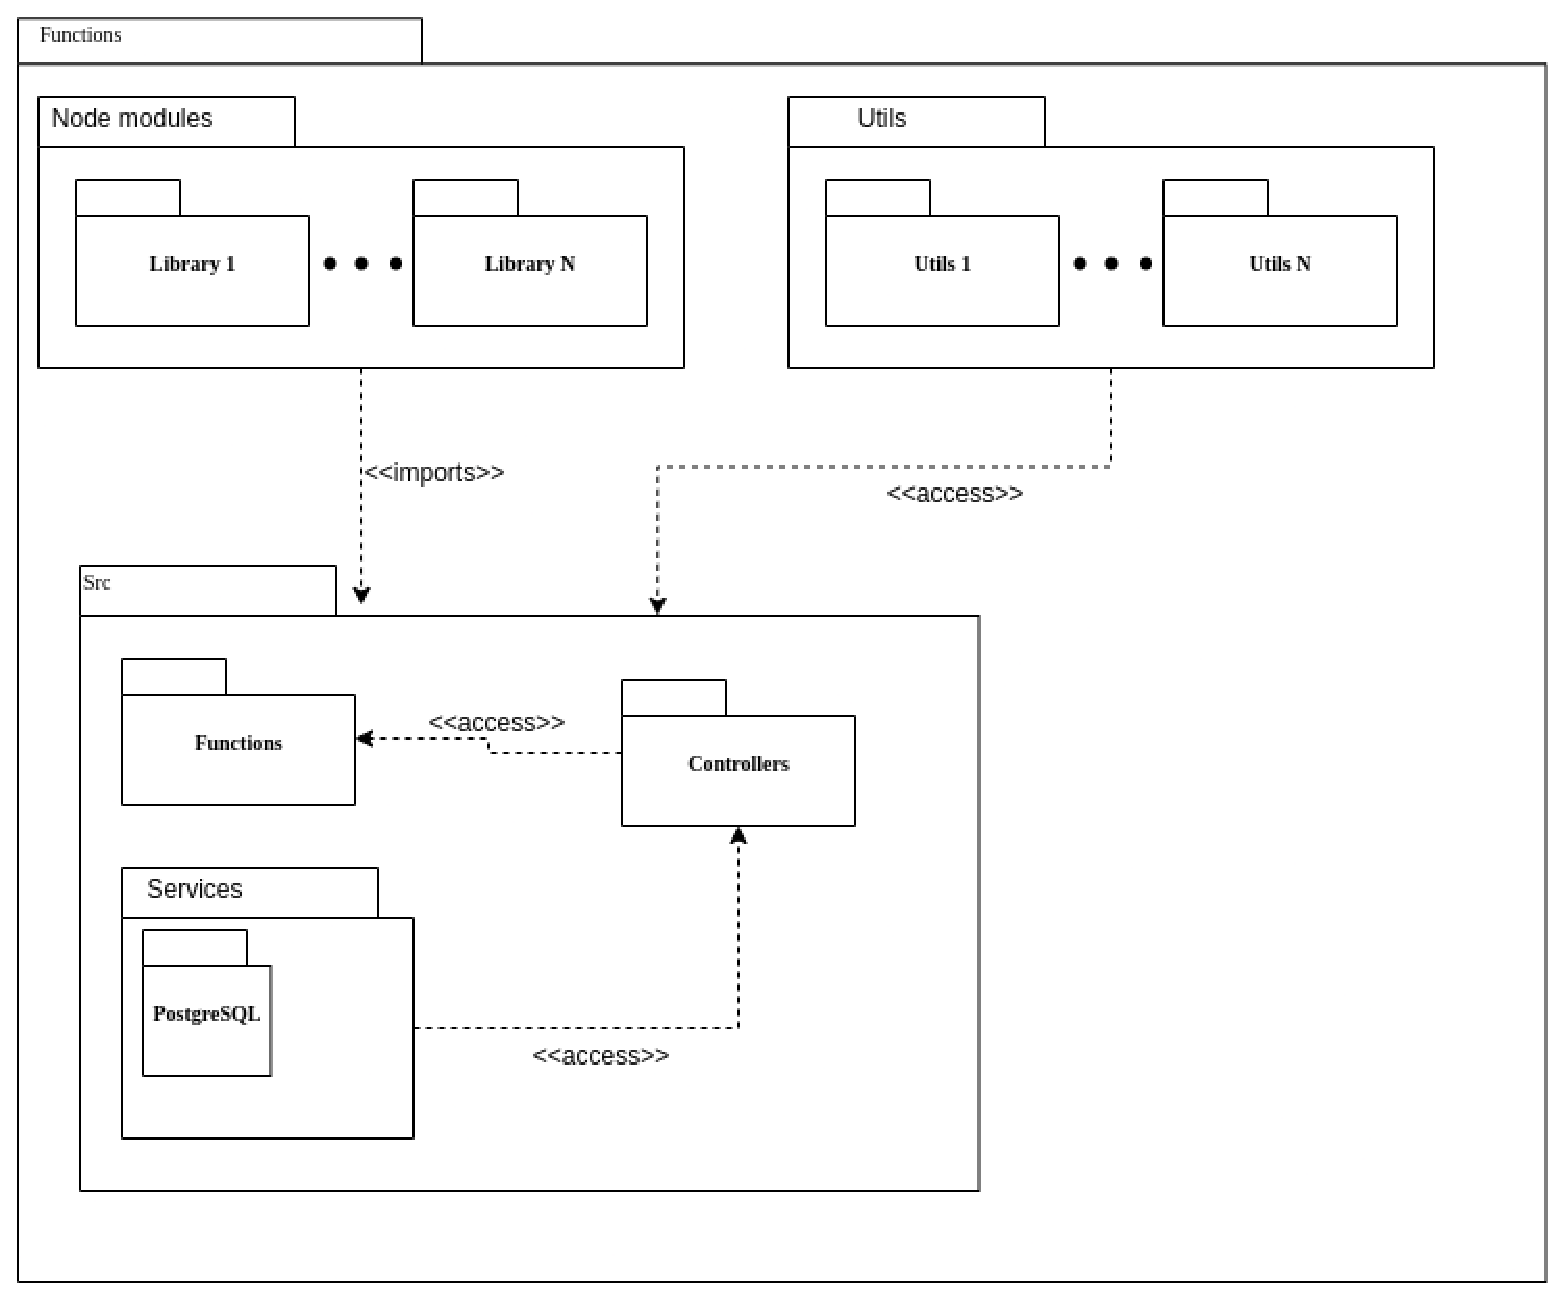
\includegraphics{figuras/content.eps}}
	\caption{Diagrama de Pacotes \textit{Content Server}}
	\label{fig08}
\end{figure}
\begin{figure}[h!]
	\centering
	\resizebox{0.6\textwidth}{!}{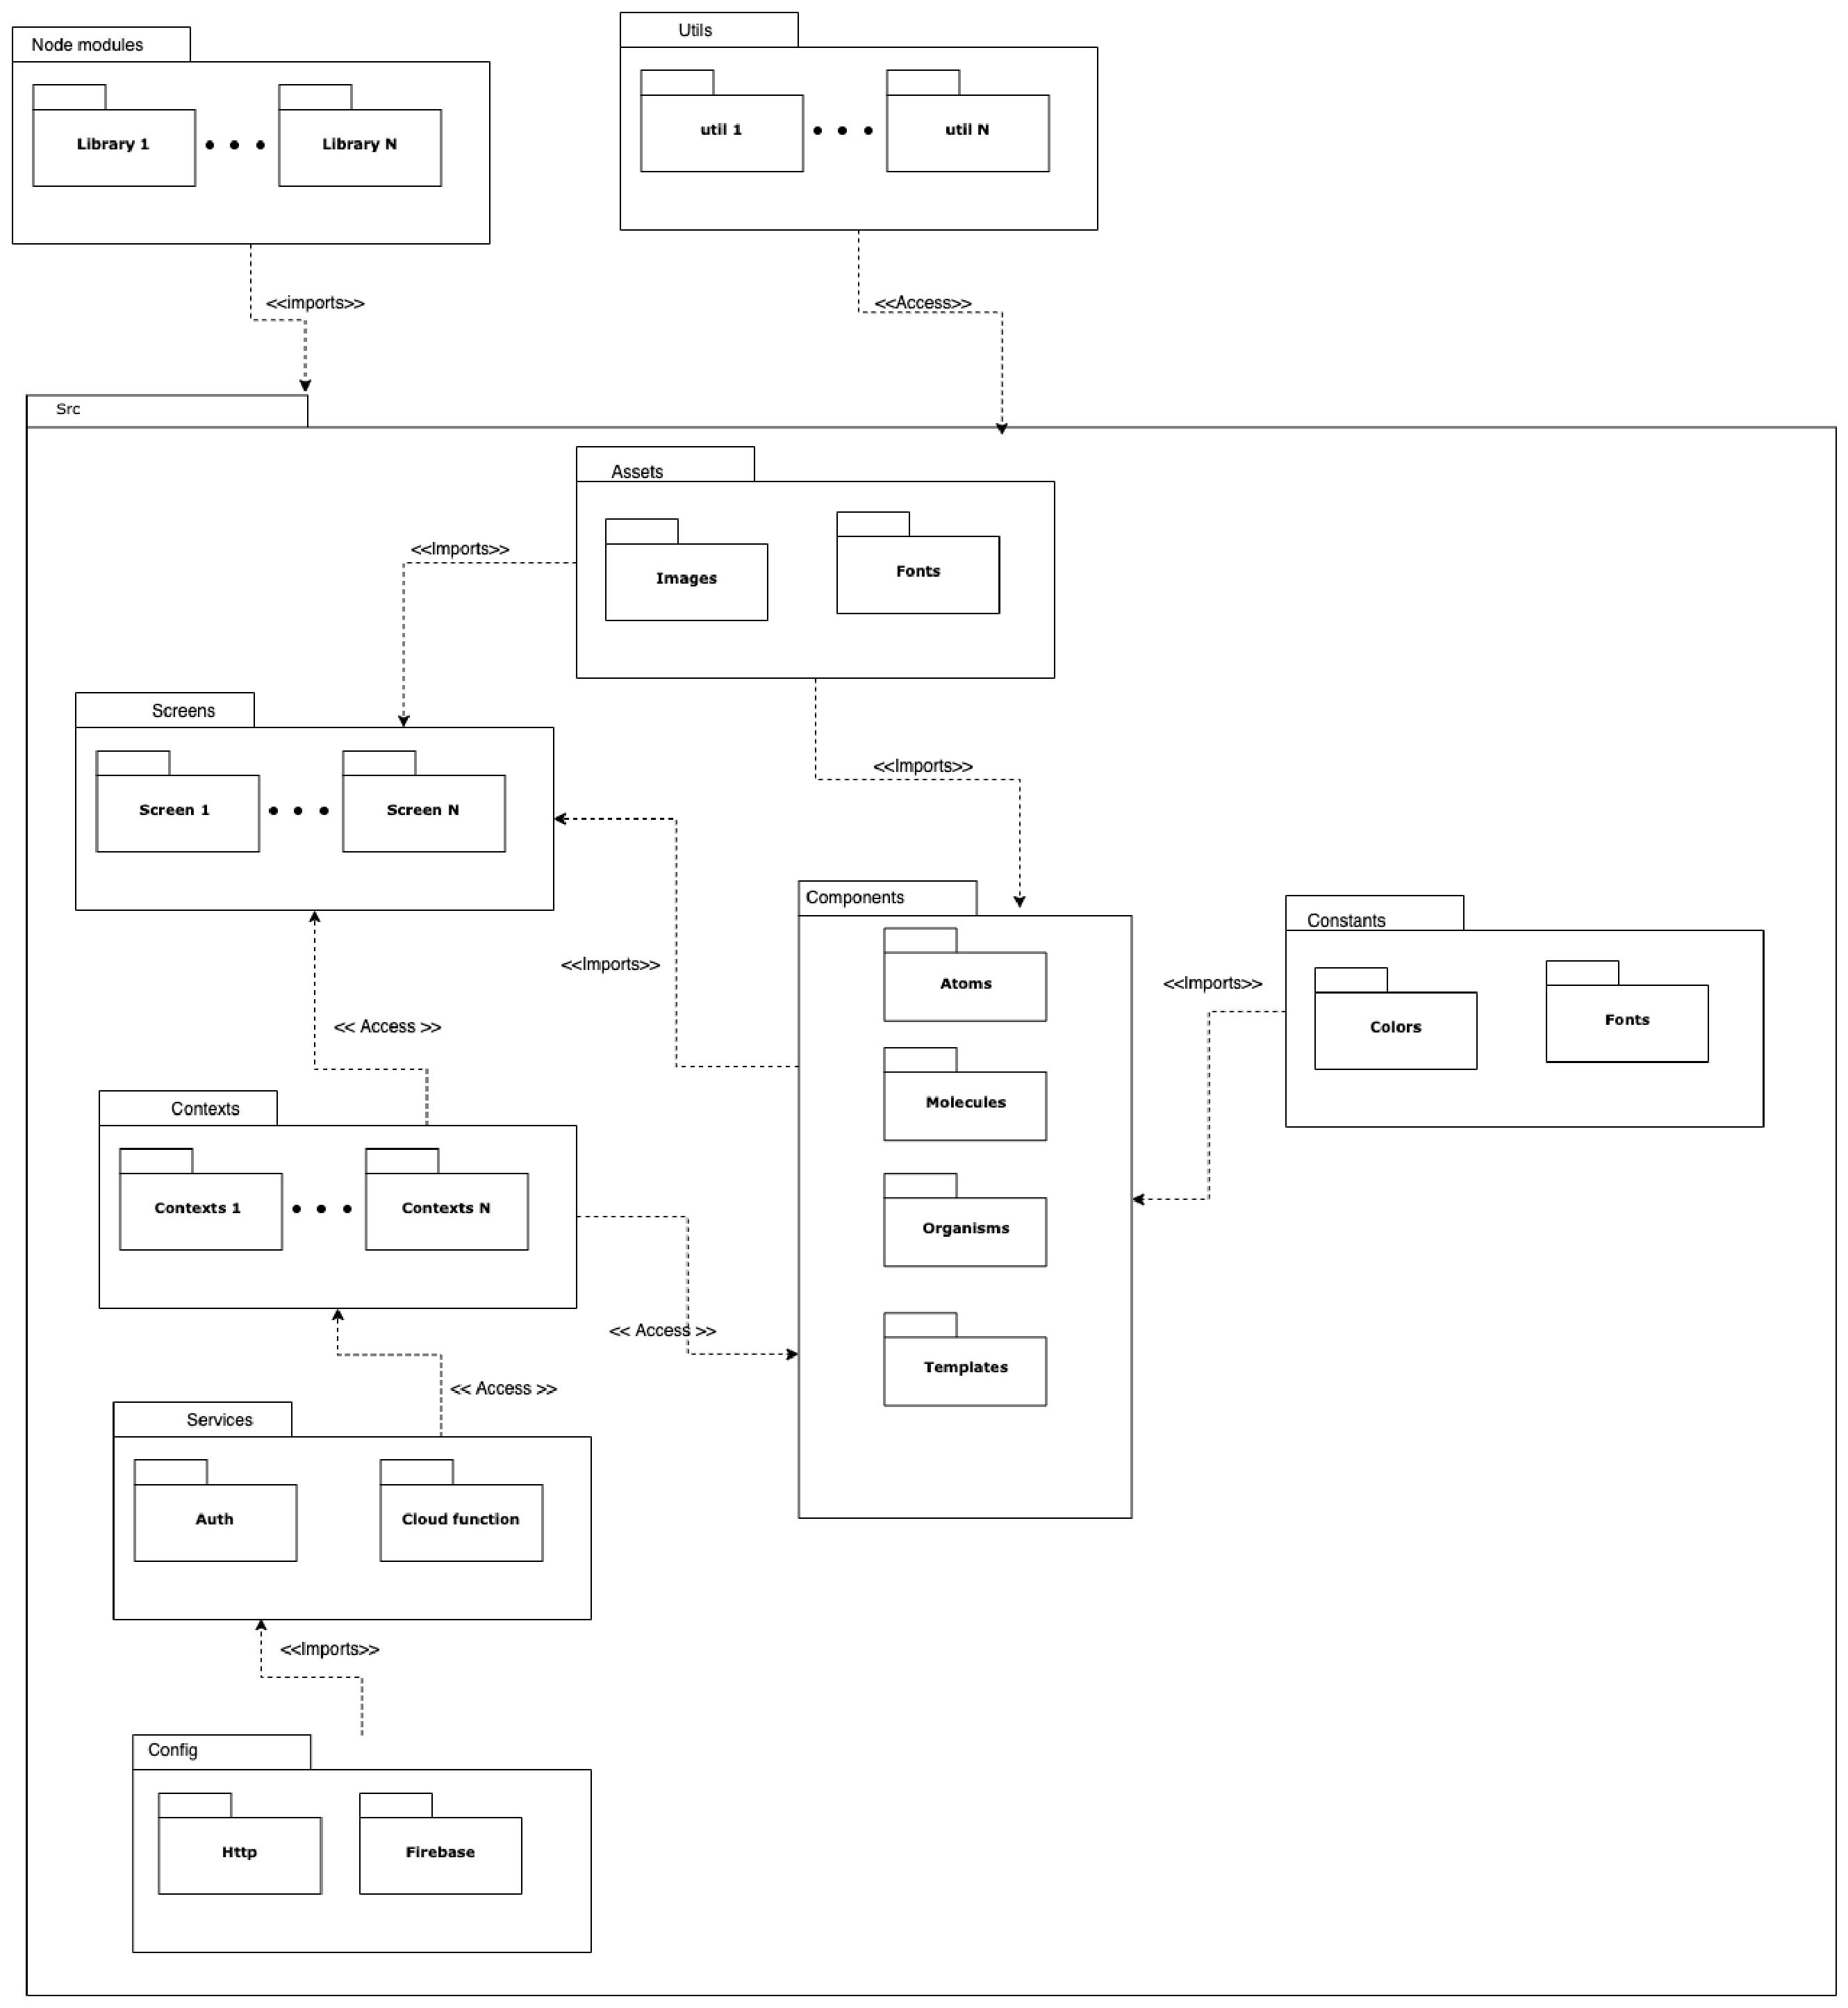
\includegraphics{figuras/frontend.eps}}
	\caption{Diagrama de Pacotes \textit{Frontend}}
	\label{fig09}
\end{figure}

\begin{figure}[h!]
	\centering
	\resizebox{0.5\textwidth}{!}{\includegraphics{figuras/assets.eps}}
	\caption{Diagrama de Pacotes \textit{Files Server}}
	\label{fig10}
\end{figure}

\subsection{Público-Alvo}
\label{Publico-Alvo}
A Lean Inception foi utilizada como forma de alinhar os desenvolvedores e \textit{stakeholders} em relação ao aplicativo antes de sua execução e confirmar sua viabilidade e necessidade. O processo aborda a visão do produto, a compreensão de personas, suas jornadas de usuário e 
o desenvolvimento de funcionalidades de alto nível \cite{lean}. No estágio de definição da visão do produto, a equipe e \textit{stakeholders} do projeto responderam questões relativas ao público alvo da aplicação, o objetivo e principais características, como pode ser visto nas 
Figuras \ref{fig11} e \ref{fig12}. 

\begin{figure}[h!]
	\centering
	\resizebox{0.85\textwidth}{!}{\includegraphics{figuras/visao_produto.eps}}
	\caption{Visão de Produto}
	\label{fig11}
\end{figure}

\begin{figure}[h!]
	\centering
	\resizebox{1\textwidth}{!}{\includegraphics{figuras/produto_e_nao_e.eps}}
	\caption{Definição do Produto}
	\label{fig12}
\end{figure}

Como definida no Capítulo de \hyperref[chap:Referencial]{Referencial Teórico}, as personas são representações detalhadas de perfis semifictícios e são desenvolvidas para ajudar a equipe a compreender melhor os usuários, bem como suas 
necessidades e expectativas. 

Ainda durante a Lean Inception, na fase de descrição de personas, foram criadas três personas que representam diferentes tipos de usuários do aplicativo. Essas personas foram essenciais para realizar as jornadas das personas e levantar as funcionalidades necessárias para atender às 
suas necessidades e expectativas. As Figuras \ref{fig13}, \ref{fig14} e \ref{fig15} mostram os três principais perfis levantados.

\begin{figure}[h!]
	\centering
	\resizebox{1.1\textwidth}{!}{\includegraphics{figuras/persona1.eps}}
	\caption{Persona 1}
	\label{fig13}
\end{figure}

\begin{figure}[h!]
	\centering
	\resizebox{1.1\textwidth}{!}{\includegraphics{figuras/persona2.eps}}
	\caption{Persona 2}
	\label{fig14}
\end{figure}

\begin{figure}[h!]
	\centering
	\begin{adjustbox}{center}
		\includegraphics[width=1.5\textwidth]{figuras/persona3.eps}
	\end{adjustbox}
	\caption{Persona 3}
	\label{fig15}
\end{figure}

\subsection{Guia de Estilo}
\label{Guia de Estilo}
O guia de estilo do produto foi desenvolvido a partir da criação de um Manual de Identidade Visual\footnote{Manual de Identidade Visual Multilind, 2021. Disponível
em: \url{https://fga-eps-mds.github.io/2021.1-Multilind-Docs/img/manualIdentidade/Manual_Id.pdf} (último acesso: Julho 2023)}. Esse manual definiu os elementos fundamentais da marca, incluindo cores, tipografia, aplicação da marca, símbolo e conceitos base.

O símbolo do Multilind é representado pelo beija-flor, que simboliza a pajé e a espiritualidade da língua. As principais cores presentes na logomarca são representadas pelos hexadecimais "\#04B47F" e "\#338BAE".

Além disso, outras cores foram selecionadas como base para o desenvolvimento do \textit{design} de interface da aplicação, que podem ser vistas nas Figuras \ref{fig16} e \ref{fig17}.

\begin{figure}[h!]
	\centering
	\resizebox{1\textwidth}{!}{\includegraphics{figuras/cor1.eps}}
	\caption{Cores da Aplicação}
	\label{fig16}
\end{figure}

\begin{figure}[h!]
	\centering
	\resizebox{1\textwidth}{!}{\includegraphics{figuras/cor2.eps}}
	\caption{Cores da Aplicação}
	\label{fig17}
\end{figure}

\subsection{Funcionalidades}
\label{Funcionalidades}
A versão 1.4.0 da aplicação possui diversas funcionalidades voltadas para o mapeamento e divulgação das línguas indígenas brasileiras. Entre essas funcionalidades, destaca-se o mapeamento das línguas, que permite aos usuários 
explorar através do mapa e descobrir informações sobre línguas indígenas brasileiras. Isso inclui detalhes sobre o tronco e família linguística a que a língua pertence, seu dicionário e imagens relativas a lista de palavras.

Além disso, a aplicação também oferece recursos de tradução para o português indígena e o português formal. Os usuários podem fazer buscas por palavras e visualizar informações como significado e imagens relativas.

\begin{figure}[h!]
	\centering
	\resizebox{1\textwidth}{!}{\includegraphics{figuras/app1.eps}}
	\caption{Telas da Aplicação}
	\label{fig18}
\end{figure}

\begin{figure}[h!]
	\centering
	\resizebox{1\textwidth}{!}{\includegraphics{figuras/app2.eps}}
	\caption{Telas da Aplicação}
	\label{fig19}
\end{figure}


\section{Prova de Conceito}
\label{sec:Prova de Conceito}
Com o objetivo de avaliar as melhorias propostas no aplicativo Multilind em relação a usabilidade e experiência de usuário, provas de conceito foram 
realizadas para avaliar tanto a última versão do aplicativo (v1.4.0), quanto a versão com melhorias propostas. O primeiro ciclo de testes foi realizado 
com objetivo de coletar métricas e informações de usabilidade e experiência do usuário. Já o segundo ciclo de testes visa validar as melhorias propostas e avaliar seus resultados.

Todos os testadores participaram voluntariamente, de acordo com os termos estabelecidos no Termo de Consentimento, que foi adaptado do 
modelo da Universidade de Araraquara (Universidade de Araraquara, 2023), disponível no Apêndice C para consulta.

\subsection{Primeiro Ciclo de Testes}
\label{sec:Primeiro Ciclo}
O primeiro ciclo de testes de usabilidade foi realizado com cinco testadores, que fazem parte do público alvo da aplicação. Foi realizado um teste abrangendo as sete funcionalidades 
principais do aplicativo, com o objetivo de identificar seus aspectos-chave. Durante o teste, os usuários forneceram \textit{feedback} instantâneo sobre sua percepção de cada funcionalidade testada. 

Além disso, como uma ferramenta adicional de teste de usabilidade, foi utilizado o Maze para avaliar a navegação e a facilidade de uso do aplicativo. Os testadores foram solicitados a realizar  
tarefas e o tempo necessário para concluir o percurso foi registrado. Essa abordagem permitiu identificar eventuais dificuldades de navegação e fornecer informações para aprimorar a usabilidade do aplicativo.
Após a conclusão dos testes, foi aplicado um questionário baseado no Formulário de \textit{Attrakdiff} para avaliar a experiência do usuário no aplicativo Multilind.

\begin{description}
    \item As funcionalidades testadas foram:
	\begin{itemize}
		\item F01 - Visualizar línguas através do mapa
		\item F02 - Ver detalhes de uma língua ao clicar em um ponto no mapa
		\item F03 - Visualizar línguas por ordem alfabética
		\item F04 - Visualizar línguas por família linguística
		\item F05 - Ver dicionário de palavras de uma língua específica
		\item F06 - Ver tradução de uma palavra para o português formal
		\item F07 - Visualizar imagens relativas as palavras de uma língua
	\end{itemize}
\end{description}

\subsubsection{Resultado do Primeiro Ciclo de Testes}
\label{sec:Resultado do Primeiro Ciclo de Testes}
Após finalizar o primeiro ciclo de testes, utilizando a versão mais recente da aplicação, alguns \textit{feedbacks} foram realizados pelos testadores, que incluem:

\begin{itemize}
	\item Ausência de cores: usuários relataram sentir que a aplicação carecia de uma paleta de cores mais vibrantes para torná-la visivelmente atraente.
	\item Falta de orientação no primeiro uso: foi observado pelos testadores uma falta de instruções claras e orientações sobre como navegar e utilizar as funcionalidades no primeiro acesso ao aplicativo.
	\item Maior clareza na opção de visualizar línguas por família linguística: alguns testadores relataram dificuldades em localizar a opção para visualizar as línguas agrupadas por família linguística.
	\item Carência de informações a respeito de contribuição: houve interesse manifestado por alguns testadores em contribuir com a base de dados do aplicativo, porém, sentiram falta de informações claras sobre 
	como realizar tal contribuição. 
\end{itemize}

A Tabela \ref{tab04} apresenta o tempo gasto por cada testador durante o teste de usabilidade separado por funcionalidade.

\begin{table}[h!]
	\centering
	\caption{Tempo Gasto por Testador}
	\label{tab04}
	\begin{tabular}{l|l|l|l|l|l}
	Fucionalidade & Testador 1 & Testador 2 & Testador 3 & Testador 4 & Testador 5 \\
	F01                   & 25.7s     & 109.3s     & 3.36s      & 232s       & 6.4s      \\
	F02                   & 21.2s        & 18.9s      & 6.45s      & 181.7s    & 17.2s     \\
	F03                   & 26.1s        & 25.7s      & 26.5s      & 36.9s     & 23.6s     \\
	F04                   & 69.6s        & 309.3s     & 283.2s     & 136.2s     & 193.9s     \\
	F05                   & 32.1s      & 31.4s      & 21.7s     & 72.6s     & 16.4s     \\
	F06                   & 30.7s     & 8.4s      & 24s     & 45.7s     & 75.5s     \\
	F07                   & 43.2s     & 23.8s      & 43.5s     & 181.2s    & 35s       
	\end{tabular}
\end{table}


A tabela presente no Google Sheets apresenta as avaliações obtidas por meio do formulário \textit{Attrakdiff} aplicado aos testadores do aplicativo. Além disso, as Figuras \ref{fig20} e \ref{fig21} ilustram a média de respostas geral e a média 
de respostas separadas pelas quatro dimensões principais, respectivamente.

\begin{figure}[h!]
	\centering
	\resizebox{0.85\textwidth}{!}{\includegraphics{figuras/media-geral.eps}}
	\caption{Média Geral \textit{Attrakdiff}}
	\label{fig20}
\end{figure}

\begin{figure}[h!]
	\centering
	\resizebox{0.85\textwidth}{!}{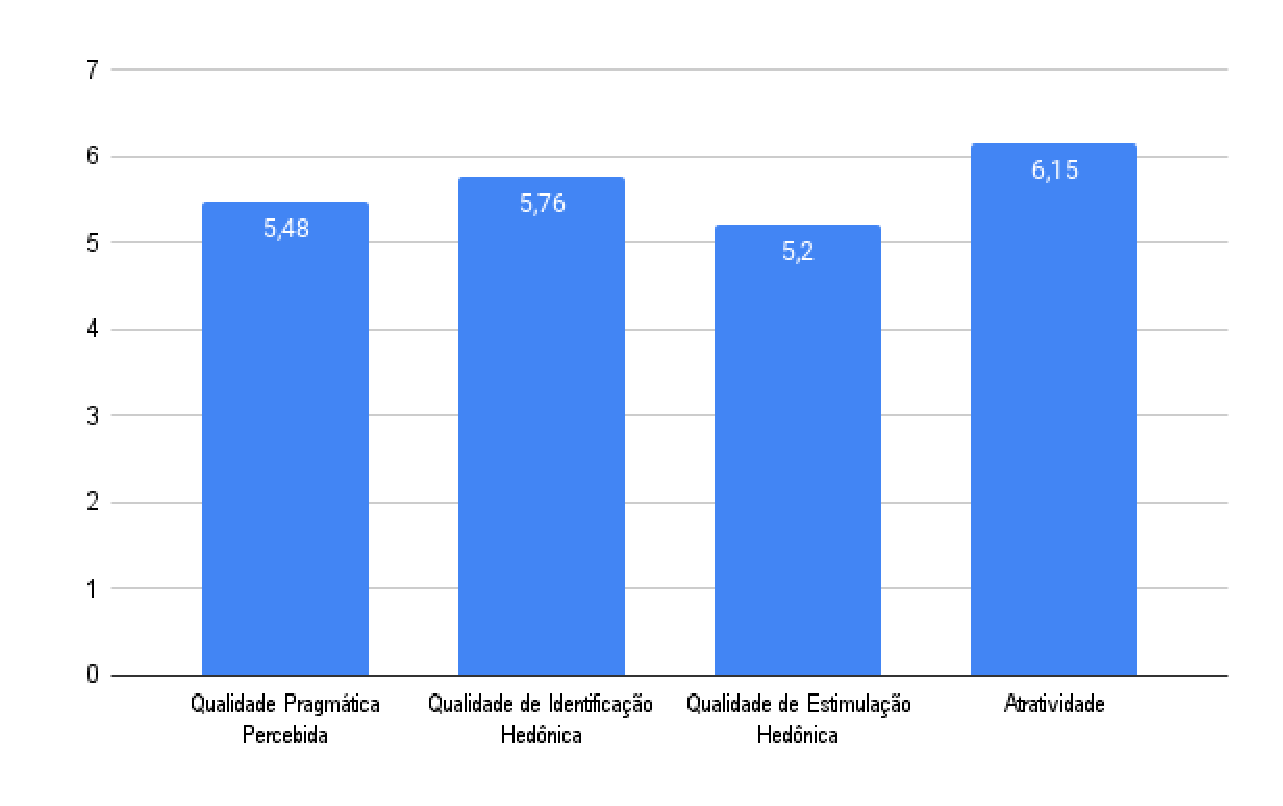
\includegraphics{figuras/media-separada.eps}}
	\caption{Média \textit{Attrakdiff} por dimensões}
	\label{fig21}
\end{figure}

\subsection{Segundo Ciclo de Testes}
\label{sec:Segundo Ciclo}
